
下面转而研究 (7.2.330.1)。
这部分与 (7.2.298.2) 的讨论平行。
具体地，得到下列严格交换的
图式~\ref{diag:7-2-25}
和图式~\ref{diag:7-2-26}。

\par\medskip\noindent\begin{minipage}{\textwidth}
\centering
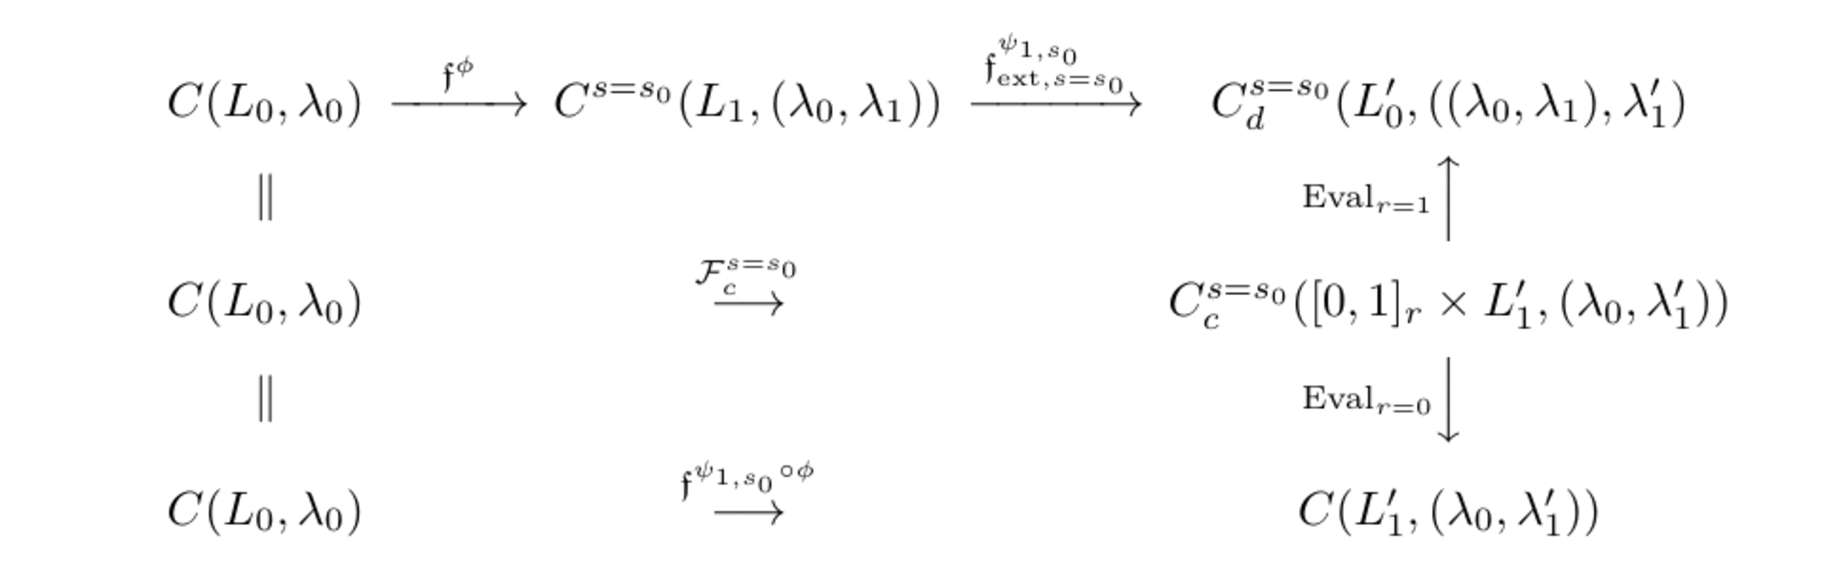
\includegraphics[width=\textwidth]{chapters/ch07-transversality/figures/phys-570-diagram-7-2-25-nocap.png}\\[0.4em]
{\renewcommand{\thefigure}{7.2.25}\refstepcounter{figure}
\normalfont\bfseries 图式~\thefigure\label{diag:7-2-25}}
\end{minipage}\par\medskip
图式~\ref{diag:7-2-25} 的标注保留原样\translatornote{原书图式 7.2.25 右上对象写
$C_d^{s=s_0}(L'_0,((\lambda_0,\lambda_1),\lambda'_1))$；
但入射的
$\mathfrak f_{\mathrm{ext},s=s_0}^{\psi_{1,s_0}}$
在图式 7.2.22 中以 $L'_1$ 为靶底空间。
此处保留源图，预期底空间为 $L'_1$。}。

\par\medskip\noindent\begin{minipage}{\textwidth}
\centering
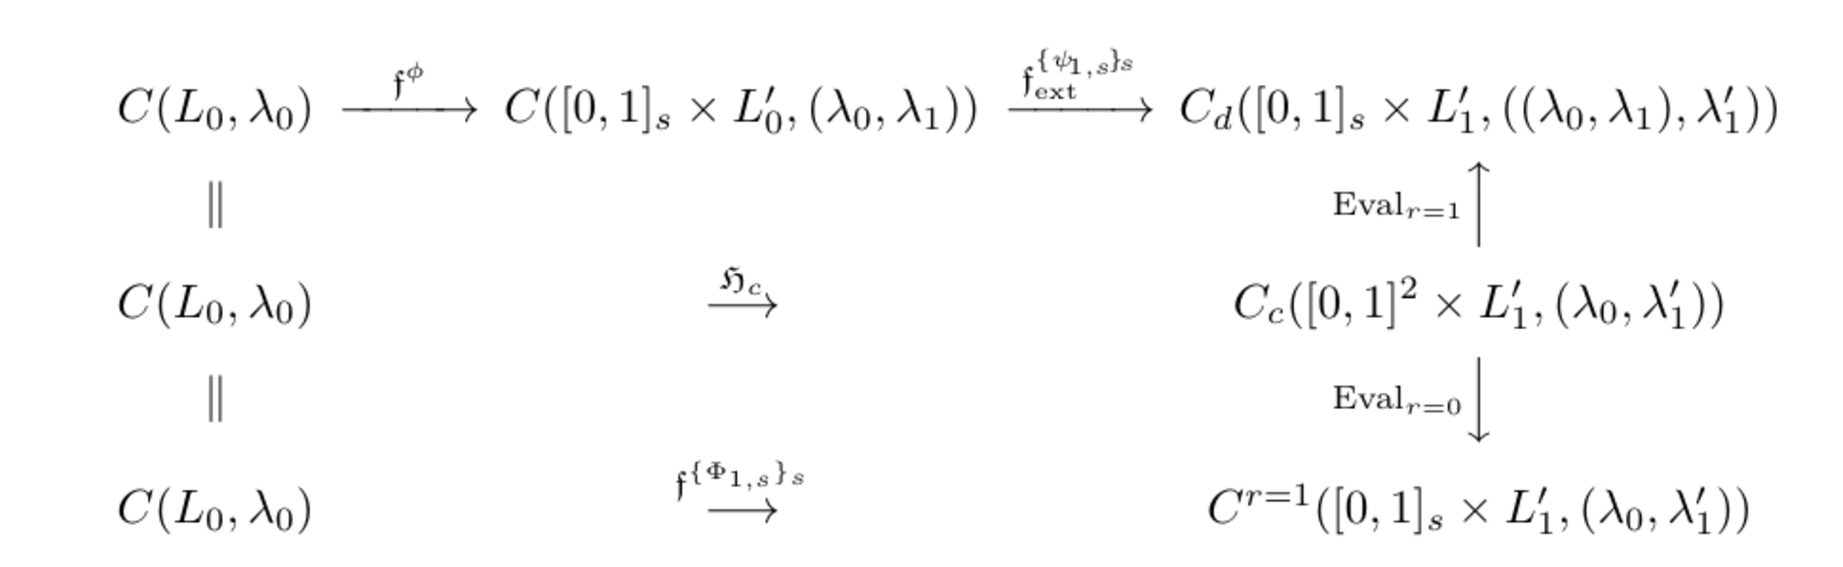
\includegraphics[width=\textwidth]{chapters/ch07-transversality/figures/phys-570-diagram-7-2-26-nocap.png}\\[0.4em]
{\renewcommand{\thefigure}{7.2.26}\refstepcounter{figure}
\normalfont\bfseries 图式~\thefigure\label{diag:7-2-26}}
\end{minipage}\par\medskip
图式~\ref{diag:7-2-26} 的标注亦保留原样\translatornote{原书图式 7.2.26 上行中点
$C([0,1]_s\times L'_0,(\lambda_0,\lambda_1))$
接 $\mathfrak f^\phi$；
按图式 7.2.25 及既定靶空间，
底空间应为 $L_1$。
右下对象又标 $C^{r=1}$，
而入射箭头标 $\operatorname{Eval}_{r=0}$；
它与图式 7.2.21 的相反标注互为镜像。
两处均保留源图，端面模型名待核。}。

至此，分别完成了
(7.2.280.1)、(7.2.280.2)
和 (7.2.280.3) 三种情形的讨论。
现在把它们胶合起来，
得到所需的同伦的同伦 $\mathfrak H$。

先回顾命题~\ref{prop:4-2-37}
的证明中已经用过的构造。
设 $\mathfrak C_j$（$j=1,2$）
各自是
$[0,1]_r\times C$
或 $[0,1]^2\times C$ 的模型。
假设 $\mathfrak C_1$ 的
$\operatorname{Eval}_{r=1}$ 的靶
与 $\mathfrak C_2$ 的
$\operatorname{Eval}_{r=0}$ 的靶相同。
定义胶合代数\translatornote{原书这一定义的右侧写成
$(\operatorname{Eval}_{r=0})_1(y)$；
但 $y$ 属 $\mathfrak C_2$，
且本段首句已指定接合的是
$\mathfrak C_2$ 的 $r=0$ 评价，
故此处下标应为 $2$。}：
\[
\begin{aligned}
\mathfrak C_1\vee_r\mathfrak C_2
=\bigl\{(x,y)\in\mathfrak C_1\oplus\mathfrak C_2\mid
&(\operatorname{Eval}_{r=1})_1(x)\\
&=(\operatorname{Eval}_{r=0})_2(y)\bigr\}.
\end{aligned}
\]
复形 $\mathfrak C_1\vee_r\mathfrak C_2$
具有滤过 $A_{n,K}$ 代数结构。
这是因为当
$(k,\beta)\ne(1,\beta_0)$ 时，
评价映射的分量
$(\operatorname{Eval}_{r=r_0})_{k,\beta}$
为零；由此容易验证闭合性。

在 $\mathfrak C_1\vee_r\mathfrak C_2$
上定义端点评价为
\[
\operatorname{Eval}_{r=0}(x,y)
=\operatorname{Eval}_{r=0}(x),\qquad
\operatorname{Eval}_{r=1}(x,y)
=\operatorname{Eval}_{r=1}(y).
\]
在下文的应用中，
对每个 $j=1,2$，
$\mathfrak C_j$
均为
\[
[0,1]^2\times
\bigl(C_0,\{C_{j;r_0,s_0}\}_{r_0,s_0}\bigr)
\]
的模型，
且
$C_{1;r_0=1,s_0}
=C_{2;r_0=0,s_0}$。
此时
\[
\operatorname{Incl}\colon
C_0\longrightarrow\mathfrak C_1\vee_r\mathfrak C_2
\]
由
$\operatorname{Incl}(x)
=(\operatorname{Incl}(x),\operatorname{Incl}(x))$
定义。

若
$\mathfrak f_i\colon C\to\mathfrak C_i$
是滤过 $A_{n,K}$ 同态，
并满足
$\operatorname{Eval}_{r=1}\circ\mathfrak f_1
=\operatorname{Eval}_{r=0}\circ\mathfrak f_2$，
则可定义滤过 $A_{n,K}$ 同态
\[
\mathfrak f_1\vee_r\mathfrak f_2\colon
C\longrightarrow
\mathfrak C_1\vee_r\mathfrak C_2,
\qquad
(\mathfrak f_1\vee_r\mathfrak f_2)_{k,\beta}
=(\mathfrak f_1)_{k,\beta}
\oplus(\mathfrak f_2)_{k,\beta}.
\]
同法可胶合多于两个代数及同态。

现在把迄今构造的五个同伦的同伦中的三个胶合起来。
